\chapter{Introduzione alle carte vettoriali}

\section{Importare un layer vettoriale}
	Un formato vettoriale abbastanza comune in un GIS è lo SHAPE file, il cui standard è stato definito dall'ESRI. GRASS supporta una moltitudine di formati\footnote{Di default, i seguenti: ESRI Shapefile (read/write) MapInfo File (read/write) UK .NTF (readonly) SDTS (readonly) TIGER (read/write) S57 (read/write) DGN (read/write) VRT (readonly) REC (readonly) Memory (read/write) BNA (read/write) CSV (read/write) GML (read/write) GPX (read/write) KML (read/write) GeoJSON (read/write) Interlis 1 (read/write) Interlis 2 (read/write) GMT (read/write) SQLite (read/write) ODBC (read/write) PGeo (readonly) OGDI (readonly) PostgreSQL (read/write) MySQL (read/write) XPlane (readonly) AVCBin (readonly) AVCE00 (readonly) Geoconcept (read/write).}, molti dei quali sono apprezzabili dal menù \textsf{$\text{File}\rightarrow\text{Import vector map}$}. Se non si riconosce il formato da importare tra quelli elencati, è possibile utilizzare per l'importazione la libreria OGR (\textsf{$\text{Filei}\rightarrow\text{Import~vector~map}\rightarrow\text{Import~vector~data~using~OGR}$}).
	Se in una sola cartella sono disponibili molti SHAPE file da importare contemporaneamente, è possibile farlo usando la voce \textsf{Multiple vector data import using OGR}.

	Supponendo di voler importare un solo file:
	
	\begin{itemize}
		\item \textsf{$\text{File}\rightarrow\text{Import~vector~map}\rightarrow\text{Import~vector~data~using~OGR}$};
		\item nella finestra che appare, nella scheda \textsf{Required} selezioniamo il file da importare e diamo un nome al layer; se viene spuntata l'opzione \textsf{Add created map into layer tree }nella parte inferiore della finestra, il layer importato verrà automaticamente aggiunto a quelli visualizzati nel Map Display;
		\item nella scheda \textsf{Selection} è possibile definire i nomi dei layer dello SHAPE file che vogliamo importare, operando una selezione; se nessun nome verrà elencato, tutti i layer disponibili nello SHAPE file saranno importati; è possibile ottenere una lista dei layer disponibili nel file andando nella scheda \textsf{Optional} e spuntando \textsf{List available layers in data source and exit}, premendo dopo \textsf{Run}.
		\item la scheda \textsf{Subregion} offre l'opportunità di importare, da uno SHAPE file di grande estensione geografica, solo i dati per la region attualmente in uso, semplicemente spuntando l'opzione apposita; la casella di testo permette di selezionare, tra molte sub-region salvate in GRASS, quelle che devono essere importate dallo SHAPE.
		\item al termine, premere \textsf{Run}: compiuta l'operazione, il nuovo layer vettoriale sarà disponibile nel Layer Manager. Per renderizzarlo nella mappa, andare nel Map Display e premere il pulsante \textsf{Display map }(il primo da sinistra).
	\end{itemize}

	\subsection{Caricare layer in un nuovo workspace}
		In qualsiasi momento è possibile caricare all'interno del workspace in GRASS i layer presenti nei mapset che fanno capo alla location corrente, aggiungendoli quindi nel proprio Layer Manager. Si può avere necessità di caricare dei layer perché si è dimenticato di spuntare l'opzione \textsf{Add created map into layer tree} in fase di importazione, o perchè si è avviato un nuovo workspace, o perchè non sono state salvate le impostazioni del workspace sul quale si stava lavorando precedentemente.

		Per caricare i layer, utilizzare la voce di menù \textsf{$\text{File}\rightarrow\text{Workspace}\rightarrow\text{Load map layers}$}; si potranno quindi selezionare i layer da caricare nel Layer Manager scegliendo tra \emph{raster} e \emph{vector}, all'interno dei mapset della location in uso.


	\subsection{Proprietà di un layer vettoriale}
		È possibile accedere alle proprietà di un layer facendo click con il tasto destro del mouse sul layer all'interno del Layer Manager.  Da questo menù è possibile definire alcune proprietà, come il nome del layer (\textsf{Rename}) o la sua stessa presenza all'interno del Layer Manager (\textsf{Remove}); è inoltre possibile cambiare il livello di opacità del layer rispetto al resto della mappa (\textsf{Change opacity level}). Facendo click su \textsf{Zoom to selected map} lo zoom del Map Display viene modificato per visualizzare il layer nella sua interezza.

		Comunque, la finestra delle proprietà del layer è accessibile facendo click su \textsf{Properties} (che avvia il modulo \textsf{d.vect}). Viene mostrata in automatico la scheda \textsf{Selection}, che permette di definire ciò che deve essere visualizzato, per quel layer, sulla mappa.
		
		\begin{description}
			\item [{Selezionare~geometrie}] In particolare, può accadere che siano selezionate di default tutte le geometrie, compresi i centroidi: se la visualizzazione della mappa appare ``sporcata'' da troppi punti, è probabile che si voglia deselezionare la voce sui centroidi e aggiornare la visualizzazione nel Map Display.
			\item [{Selezionare~layer}] In un vettoriale, ad ogni layer viene attribuito un numero, e di default tutti i layer vengono visualizzati nella mappa, come si può notare nella box \textsf{Layer number }(il valore -1 visualizza tutti i layer); dal menù a tendina è possibile selezionare un layer da visualizzare.
		\end{description}
		
		Le schede successive gestiscono i colori del layer (\textsf{Colors}), le linee (\textsf{Lines}), i simboli (\textsf{Symbols}), le etichette (\textsf{Labels}) ed alcuni valori opzionali (\textsf{Optional}). È possibile applicare le modifiche senza chiudere la finestra del modulo \textsf{d.vect} (nel caso si vogliano applicare altri cambiamenti) semplicemente premendo il pulsante \textsf{Applica} al posto di \textsf{OK}, e aggiornando la visualizzazione sulla mappa.
		
		\begin{description}
			\item [{Modificare~un~layer~vettoriale}] GRASS integra una funzione di \emph{editing}, ovvero di redazione, modifica dei punti e degli attributi del layer vettoriale; è possibile accedere a questa modalità facendo click con il tasto destro del mouse sul layer nel Layer Manager e selezionando \textsf{Start editing}. Verrà portato in primo piano il Map Display, in cui è apparsa una barra degli strumenti per la modifica dei vettoriali; anche la mappa ha cambiato aspetto, e vengono visualizzate adesso tutte le geometri facenti parte del dato vettoriale, come i punti e le linee. È possibile interrogare velocemente le geometrie per vedere gli attributi ad esse associate facendo prima click sul pulsante \textsf{Display/update attributes} e poi sulla geometria di nostro interesse.

			I pulsanti di modifica sono facilmente qualificabili dal colore delle icone: tutte le icone con la stella bianca su sfondo giallo aggiungono una geometria, quelle con la freccia bianca su sfondo blu spostano le geometrie, quelle con una X bianca su sfondo rosso eliminano le geometrie.

			Nella parte iniziale della barra di modifica delle geometrie è presente anche un menù a tendina che permette di cambiare agevolmente il layer di lavoro (scegliendone uno tra quelli elencati nel Layer Manager).
		\end{description}

	\subsection{Visualizzare etichette da un layer vettoriale}
		Può essere utile, a fini divulgativi o di studio, visualizzare gli attributi delle geometrie accanto a queste all'interno della mappa, soprattutto nel caso in cui questi attributi siano stati memorizzati nel file vettoriale sotto forma di testo. Un esempio pratico è un file dei punti di quota, i cui valori testuali saranno immagazzinati in una colonna del database che affianca le geometrie. La visualizzazione degli attributi nella mappa è frutto della modifica di alcune impostazioni nelle proprietà del layer vettoriale:
		
		\begin{itemize}
			\item fare click con il tasto destro del mouse sul layer di nostro interesse all'interno del Layer Manager e aprire la finestra delle proprietà selezionando la voce \textsf{Properties};
			\item nella scheda \textsf{Labels} impostare dal menù a tendina \textsf{Name of column to be displayed} il nome della colonna del database contenente le informazioni da visualizzare;
			\item è possibile impostare alcune opzioni come il colore dell'etichetta, dello sfondo di questa e del bordo, oppure deciderle di rendere queste ultime due caratteristiche trasparenti; la dimensione dell'etichetta può essere impostata tramite il valore in \textsf{Label size (pixels)} ed il nome del font con cui disegnare le etichette deve essere inserito nell'apposita casella \textsf{Font name:} (si consiglia di inserire \textsf{romans}, che è il font che viene visualizzato più velocemente all'interno di GRASS\footnote{Altri font disponibili sono cyrilc, gothgbt, gothgrt, gothitt, greekc, greekcs, greekp, greeks, italicc, italiccs, italict, romanc, romancs, romand, romans, romant, scriptc, scripts.}); è inoltre possibile definire la giustificazione orizzontale e verticale dell'etichetta rispetto alla geometria di appartenenza, tramite i menù a tendina rispettivamente \textsf{Label horizontal justification} e \textsf{Label vertical justification};
			\item passare alla scheda \textsf{Optional} e selezionare, nella box \textsf{Display}, anche la voce \textsf{attr} (questa impostazione serve a permettere che nel Map Display vengano visualizzate anche le informazioni degli attributi così come definite in \textsf{Labels}). Quindi, premere \textsf{Run}.
		\end{itemize}

\section{Importare un vettoriale da AutoCAD}
	AutoCAD è un software CAD (\emph{Computer Aided Design} o \emph{Computer Aided Drafting}) di disegno 2D e 3D sviluppato e venduto da Autodesk, Inc., entrato nel mercato nel 1982. Viene attualmente utilizzato, in molti ambiti di rilievo archeologico, per archiviare dati relativi agli scavi, salvando le informazioni nel formato proprietario \emph{dwg}. Nel 1982 la Autodesk ha anche sviluppato un formato di dati CAD compatibile con AutoCAD, il \emph{dxf}, rivelandone la sintassi, permettendo così agli sviluppatori di altri software (anche open source) di poter importare i dati creati con AutoCAD in altri software, o esportare i dati creati con altri programmi su AutoCAD.

	\begin{table}
		\centering
		$\xymatrix@C=50pt{*+[F]{dwg}\ar[r]^{pulizia} & *+[F=]{dxf}\ar[r] & *+[F-,]{layer~GRASS}}$
		\caption{{\small Workflow schematico dell'importazione dei dati da CAD al GIS.}}
	\end{table}

	\subsection{La geometria archeologica nei CAD}
		Oggi il formato dxf è oggi uno standard \emph{de facto} per lo scambio di dati CAD tra varie applicazioni, tra cui anche GRASS, che ne integra il supporto. Lo svantaggio dei dati CAD rispetto all'impostazione ``GIS'' per la gestione dell'informazione geografica, come abbiamo visto in \textsection\ref{par:GRASS-=0000E8-ordinato}, è che non possono dirsi propriamente \emph{georeferenziati}, poichè qualsiasi geometria disegnata in un CAD in realtà è localizzata all'interno di un sistema di riferimento interno al file, più precisamente all'interno di una coppia di assi cartesiani XY avente origine nell'angolo in basso a sinistra del foglio di lavoro; ciò significa che ogni punto all'interno del CAD è descritto da una coppia di coordinate non geografiche.  Inoltre, i dati CAD mal si prestano alla memorizzazione di informazioni aggiuntive (potremmo quindi dire che i dati CAD sono quasi essenzialmente rappresentati da geometrie e non da attributi), al contrario di formati usati nei GIS, come lo SHAPE file. Questa situazione si è col tempo accompagnata alla separazione della documentazione elettronica dello scavo (geometrie) da quella cartacea (schede di unità stratigrafica, che costituiscono i naturali attributi delle geometrie). Un GIS archeologico può ovviare a questa situazione, rendendo le schede di US \emph{spatially enabled}, ovvero fondendo in un unico sistema l'aspetto geografico e quello documentativo, con evidenti vantaggi in termini di tempo e denaro risparmiati nella gestione del dato (in particolar modo se si fa utilizzo di software libero ed open source).

	\subsection{Pulire un file CAD}

		\begin{wrapfigure}{o}{0.35\columnwidth}
			\centering
			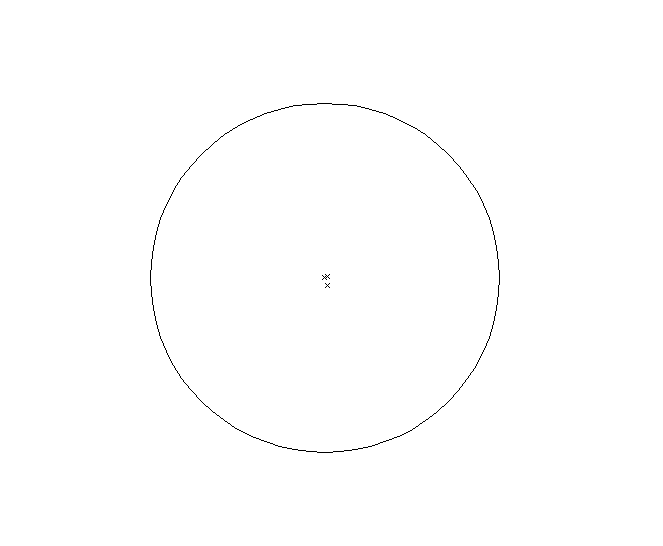
\includegraphics[scale=0.25]{img/segno}
			\caption{{\small Uno dei simboli usato all'interno del CAD per segnare la presenza di un reperto, o una quota. L'importazione senza ``pulizia'' del dxf porta ad ottenere delle geometrie che sporcano il disegno.}}
		\end{wrapfigure}
		
		Il disegno in CAD è spesso molto diverso per impostazione da un GIS; l'impossibilità dei file CAD di contenere informazioni (attributi) in un file di database associato porta spesso a disegnare o a scrivere tali informazioni nello stesso foglio di lavoro CAD. Ad esempio, è possibile trovare un layer delle quote di un rilevo archeologico effettuato in CAD, in cui ogni quota è segnata con un pallino ed una X; in altre parole, alla semplice etichetta riportante il valore della quota, è stato affiancato un disegno grafico che non rappresenta un oggetto reale, ma aiuta nella comprensione di una caratteristica del rilievo.  La mancata rimozione di tale simbolo grafico prima dell'importazione del file in un GIS conduce a grossi disagi durante l'elaborazione dei dati, in quanto queste figure dovranno essere necessariamente rimosse per ottenere un layer GIS preciso. L'esempio delle quote è molto utile per spiegare anche come, in un GIS, non ci sia bisogno di disegnare manualmente i simboli da associare ad un punto (per evidenziarne alcune caratteristiche o la presenza), poichè è sufficiente definire tale simbologia nelle proprietà del layer, ed il simbolo definito verrà associato automaticamente a tutti i punti del layer, e potrà alla stessa maniera essere rimosso in qualsiasi momento.

		Quindi, prima di procedere con l'esportazione in dxf, è necessario assicurarsi che siano stati eliminati dal disegno CAD tutte le linee e i poligoni che non rappresentino un oggetto reale all'interno del rilievo.

	\subsection{Importare un file dxf\label{sub:Importare-un-file-dxf}}
		In un primo momento, considerata la natura dei dati CAD, l'importazione di questi in GRASS può avvenire solo in una location con sistema di riferimento XY (si veda in merito quanto detto in \textsection\ref{sub:Definire-una-location}).

		\input{tab/box_limiti_dxf}

		L'importazione di dati da un software CAD è facilitata dalle molte funzioni messe a disposizione da GRASS. Il processo è il seguente:
		
		\begin{itemize}
			\item creare una nuova location con sistema di riferimento XY;
			\item dopo averla avviata, dal Layer Manager selezionare \textsf{$\text{File}\rightarrow\text{Import vector map}\rightarrow\text{DXF import}$}, aprendo l'interfaccia del modulo \textsf{v.in.dxf};
			\item nella scheda \textsf{Required} selezionare il file da importare; la scheda \textsf{DXF layers} permette, spuntando l'opzione \textsf{List available layers and exit} e premendo \textsf{Run} di elencare semplicemente tutti i layer presenti nel file (che verranno mostrati nel \textsf{Commad output}); nella stessa scheda, l'opzione \textsf{Import all objects into one layer} consente di ``fondere'' tutti gli oggetti in un unico layer e di importarli come tali. Ulteriori opzioni possono essere selezionate nella scheda \textsf{Optional} tra cui molto importante è l'attribuzione di un nome al layer, che altrimenti non può essere importato.
			\item non appena definite le varie opzioni (ricordandosi eventualmente di spuntare l'opzione in basso \textsf{Add created map into layer tree}), fare click su \textsf{Run}; nel \textsf{Command output} è possibile seguire lo stato dell'importazione e leggere le segnalazioni di eventuali errori.
		\end{itemize}

			\paragraph{Semplificare l'importazione di molti layer vettoriali}
			Esiste una maniera semplice per importare file dxf contenenti molti layer, selezionando esattamente quali importare, la voce di menù \textsf{$\text{File}\rightarrow\text{Import vector map}\rightarrow\text{Multiple DXF layers import}$}, facente sempre capo al modulo \textsf{v.in.dxf}. Selezionandola, si aprirà una finestra in cui è possibile, dopo aver selezionato il file da importare, spuntare tra i layer del file solo quelli da importare, operano così una selezione.

			\input{tab/box_importare_st}

\section{Georeferenziare una carta vettoriale}
	Le operazioni da svolgere per rettificare e georeferenziare una carta vettoriale sono simili a quelle già viste per effettuare la stessa procedura con le carte raster, in \textsection\ref{sec:Georeferenziare-una-carta-raster}, ma meno automatizzate.

	Prima di cominciare, occorre indagare l'origine della carta vettoriale da georeferenziare. Infatti, è possibile parlare di georeferenziazione solo se la carta è proiettata secondo un qualsiasi sistema di riferimento, che deve essere noto. Ad esempio, se il vettoriale è stato ricalcato da cartografia italiana realizzata negli ultimi anni, è molto probabile che sia proiettato con un sistema di riferimento Gauss-Boaga. Questo ovviamente vale anche per i file CAD distribuiti in formato dwg o dxf. In generale, è difficile che si lavori con un file CAD o comunque con un vettoriale non proiettato. Nel caso analizzato di seguito, si ha la ragionevole certezza che il vettoriale da georeferenziare è stato ricalcato da una carta UTM WGS84, per cui si procederà solo alla georeferenziazione e non alla proiezione.

	La georeferenziazione prevede anche in questo caso l'attribuzione di nuove coordinate ai punti della carta, coordinate che vengono ottenute per confronto con una carta già georeferenziata. Il modulo che si occupa di ricalcolare le coordinate della mappa in base ai punti di controllo al suolo (GPC) è \textsf{v.transform}, avviabile anche dal menù \textsf{$\text{Vector}\rightarrow\text{Develop~vector~map}\rightarrow\text{Reposition~vector~map}$}.

	Volendo riassumere, i passaggi da affrontare simili a quelli visti precedentemente sono:
	
	\begin{enumerate}
		\item importare la mappa nella propria location (in questo caso con sistema di riferimento UTM WGS84);
		\item importare all'interno di questa la carta vettoriale; se la carta non georeferenziata non ha al suo interno informazioni sulla proiezione, bisogna avere l'accortezza di mettere il segno di spunta sull'opzione \textsf{Override dataset projection (use location's projection)} del modulo \textsf{v.in.ogr}. altrimenti l'importazione fallirà.

		Da questo punto in poi, per una carta raster avremmo definito un gruppo ed un target prima di catturare i punti di controllo; per le carte vettoriali, non esiste una funzione semi-automatica per la cattura dei punti di controllo al suolo, quindi dovremo procedere a mano.

		\item aprire un altra istanza di GRASS, avviare in un nuovo map display la carta non georeferenziata;
		
		\item in un editor di testo, aprire un nuovo file di testo e riportare per almeno tre punti della carta le coordinate rispettivamente sulla carta non georeferenziata e su quella georeferenziata; per farlo è possibile premere il pulsante \textsf{Query raster/vector map(s) (display mode)} nella barra degli strumenti del map display; facendo click in un punto della carta, si otterrà nel layer manager un output simile al seguente:

		\begin{Verbatim}
			v.what --q -a map=carta_archeologica_ripos@PERMANENT //
			east_north=15.892881,41.61015 distance=0.000286
			East: 15:53:22.0308E North: 41:36:30.2112N
			Map: carta_archeologica_ripos
			Mapset: PERMANENT
			[...]
		\end{Verbatim}
		
		Nel codice sopra è stata evidenziata la posizione delle coordinate del punto nostro interesse, che dovranno essere riportate nel file, sostituendo la virgola che separa la longitudine dalla latitudine con uno spazio.

		\item Salvare il file con estensione \texttt{.points}. Il file ottenuto sarà simile al seguente:

		\begin{Verbatim}
			2663.043033 7103.878682 15.892881 41.61015
			2440.105115 6868.348733 15.892260 41.613032
			3343.564455 6694.658217 15.884017 41.60752
			3276.763815 7082.849428 15.888147 41.605921
		\end{Verbatim}
		
		Notare che le coordinate vengono riportate in formato longitudine-latitudine, ed i decimali sono separati da un punto e non da una virgola.

		\item Avviare il modulo \textsf{v.transform} e completare i due campi della scheda \textsf{Required} rispettivamente con il nome della carta da georeferenziare e con il nome che dovrà assumere quella georeferenziata; nella scheda \textsf{Optional}, alla voce ASCII file holding transform coordinates caricare il file \texttt{.points} salvato nel punto precedente, quindi avviare il processo con il pulsante \textsf{Run}.
		
		\item Al termine, sarà disponibile nell'elenco dei layer vettoriali la nuova carta georeferenziata, e sarà eventualmente possibile cancellare la vecchia.
	
	\end{enumerate}

	\input{tab/box_commentare_punti}
	
\section{Coordinate ellissoidiche e cartografiche\label{sec:Coordinate-ellissoidiche-e}}
	Può capitare che si debba importare all'interno del proprio progetto un file vettoriale georeferenziato da altre persone o con altri programmi, ed è possibile che il formato in cui le coordinate di questo file sono espresse è quello ellissoidico (ovvero il sistema di riferimento che ha come punto centrale il centro di rotazione dell'ellissoide terrestre). Per convertire le coordinate dal sistema di riferimento ellissoidico ad un sistema cartografico, è possibile utilizzare le funzionalità offerte dal software \textsf{cs2cs}, che nella distribuzione Ubuntu GNU/Linux è incluso nel pacchetto di software \textsf{gdal-bin}, che è dovrebbe essere stato precedentemente installato (si veda \textsection\ref{sec:Installazione-su-Ubuntu}). Un'interfaccia a tale software in GRASS è fornita dal modulo \textsf{g.proj}.

	Ad esempio, dato un punto di coordinate ellissoidiche lat/lon: 4606784.394 574168.739 nel sistema di riferimento italiano Gauss-Boaga, per trasformarle in coordinate lat/lon su un sistema di riferimento cartografico (in particolare WGS84), occorre dare il seguente comando da terminale:
	
	\begin{Verbatim}
		echo ``lat lon'' | cs2cs +init=epsg:32633 +to +init=epsg:4326 -f i``%.8f''
	\end{Verbatim}
	
	I punti più interessanti di questo comando sono:
	
	\begin{description}
		\item [{\texttt{lat}}] valore della latitudine di input, in questo esempio va sostituito con 4606784.394;
		\item [{\texttt{lon}}] valore della longitudine di input, in questo esempio va sostituito con 574168.739;
		\item [{\texttt{cs2cs}}] è il comando che avvia il software di conversione omonimo;
		\item [{\texttt{+init=epsg:}}] a sinistra del \texttt{+}t\texttt{o}, definisce il sistema di riferimento di input (in questo caso Gauss-Boaga fuso Est); a destra, definisce il sistema di riferimento di output (in questo caso WGS84);
		\item [{\texttt{+to}}] sigla che definisce il limite tra il sistema di riferimento di partenza e quello di destinazione della conversione;
	\end{description}
	
	L'output di questo comando, con i dati di esempio forniti, è il seguente:
	
	\begin{Verbatim}
		41.60932759     15.89013896 0.00000000
	\end{Verbatim}
	
	La prima cifra rappresenta la latitudine, seguita da longitudine ed altezza del punto (che, non essendo stata fornita nella terna di numeri di input, risulta pari a 0).
